%Define relative or absolute path of template. 
% Don´t change anything if you use the template as it is. 
\newcommand*{\MyPath}{../../tex/latex/}% 
\IfFileExists{\MyPath/AIT_report.cls}{}{\renewcommand*{\MyPath}{}}

\documentclass[
%NoTableOfContents,  % do not create a Table Of Contents
NoListOfFigures,		% do not create a List Of Figures
NoListOfTables,		% do not create a List Of Tables
language=de, 
%language=en,
]{\MyPath AIT_report}
\setboolean{FormatSlides}{false}
\setboolean{FormatScript}{true}



\usepackage{datetime}
\Company{Liebherr GmbH} % Company, is not currently used
%\SetCompanyLogo{logos/Bosch4CS} % Company logo, is not currently used
\Title{Titel hier einfügen} %Titel


%\newcommand{\Telefonnumber}{+43 664 88256044}  
%\newcommand{\Email}{amadeus.lobe@ait.ac.at}
%\newcommand{\Jobdescription}{Junior Research Engineer}

\newcommand{\Telefonnumber}{+43 664 88256085}  
\newcommand{\Email}{patrik.zips@ait.ac.at}
\newcommand{\Jobdescription}{Scientist}

%\newcommand{\TitleFirstLine}{(Teilautonome}
%\newcommand{\TitleSecondLine}{Arbeitsmaschine}

\Subject{R\ E\ P\ O\ R\ T} % preset value: report


\Author{Vorname1 Nachname1} % authos
\AuthorSecond{Vorname2 Nachname2} % authos
\AuthorThird{Vorname3 Nachname3} % authos
%\AuthorFourth{Vorname4 Nachname4} % authos
%\AuthorFifth{Vorname5 Nachname5} % authos

\AuthorText{Autoren} % preset value: Autor
%\newcommand{\Exemplarnummer}{1} % exemplar number
%\newcommand{\Versionsnummer}{1} % version number
%\Supervisor{Univ.-Prof.\@ Dr.\,techn.\@ Andreas K{\small UGI}}% Superviros, is not currently used




\DeclareTextFontCommand{\emph}{\bfseries\boldmath}
\graphicspath{{./figs/}}
%%%%%%%%%%%%%%%%%%%%%%%%%%%%%%%%%%%%%%%%%%%%%%%%%%%%%%%%%%%%%%%%%%%%%%%%%%%%%%%%%%%%%%%
% added by j.weber 26.11.2020
\usepackage{multirow}
% added by j.weber 27.11.2020
\usepackage{mathtools}
\usepackage[ruled,vlined]{algorithm2e}
% added by j.weber 28.11.2020
\usepackage{comment}

%%%%%%%%%%%%%%%%%%%%%%%%%%%%%%%%%%%%%%%%%%%%%%%%%%%%%%%%%%%%%%%%%%%%%%%%%%%%%%%%%%%%%%%
%%%%%%%%%%%%%%%%%%%%%%%%%%%%%%%%%%%%%%%%%%%%%%%%%%%%%%%%%%%%%%%%%%%%%%%%%%%%%%%%%%%%%%%
\usepackage{acronym}
\usepackage{booktabs}
\usepackage{tikz}
%\usepackage{prettyref}

\usepackage{nomencl}
\usepackage[toc]{appendix}

\usepackage{pgfplots}
\usepgfplotslibrary{groupplots}
\usetikzlibrary{pgfplots.units}
\usetikzlibrary{shapes}
\usetikzlibrary{positioning}
\usetikzlibrary{calc}
\usetikzlibrary{arrows,scopes}
\usetikzlibrary{spy}
\usetikzlibrary{decorations.pathreplacing}
\usepackage{mathrsfs}

% for (i) (ii) as items
\RequirePackage{enumerate} 
% for [H] as figure placement
\RequirePackage{float}  

%\usepackage{showframe}%frames bei subcaption

\usepackage{siunitx}
\usepackage{nicefrac}

%include todonotes
\usepackage{todonotes}
% hack to make todonotes it work with externalize
\usepackage{letltxmacro}
\LetLtxMacro{\oldmissingfigure}{\missingfigure}
\renewcommand{\missingfigure}[2][]{\tikzexternaldisable\oldmissingfigure[{#1}]{#2}\tikzexternalenable}
\LetLtxMacro{\oldtodo}{\todo}
\renewcommand{\todo}[2][]{\tikzexternaldisable\oldtodo[#1]{#2}\tikzexternalenable}


\usepackage{xcolor}

\usepackage{calc}
\usepackage[labelformat=simple]{subcaption}
\renewcommand\thesubfigure{(\alph{subfigure})}

\pgfplotsset{compat=1.16,height=0.3\textheight,legend cell align=left,tick scale binop=\times}
\pgfplotsset{grid style={loosely dotted,color=darkgray!30!gray,line width=0.6pt},tick style={black,thin}}
\pgfplotsset{every axis plot/.append style={line width=0.8pt}}

\usepgfplotslibrary{external}
% Für die Verwendung von 'external' müssen die folgenden Anpassungen in Abhängigkeit der
% LaTeX Distribution durchgeführt werden:

% fuer Texlive: pdflatex.exe -shell-escape -synctex=1 -interaction=nonstopmode %.tex
%\tikzexternalize[shell escape=-shell-escape]   % fuer TeXLive

% fuer MikTeX:  pdflatex.exe -enable-write18 -synctex=1 -interaction=nonstopmode %.tex
\tikzexternalize[shell escape=-enable-write18] % fuer MikTex

%\pgfkeys{/pgf/images/include external/.code=\includegraphics{#1}} 
%\AtBeginDocument{
%	\@ifundefined{tikzexternalrealjob}{}{%
%		\message{*** Overriding the document specification for TikZ externalizer.}%
%		\ifthenelse{\equal{\jobname}{\tikzexternalrealjob}}{}{%
%			\gdef\maketitle{}%
%		}%
%	}%
%} 

% ordner zu tikz grafiken
\tikzsetexternalprefix{graphics/pgfplots/} % Ordner muss ev. zuerst haendisch erstellt werden
%\tikzset{external/up to date check=simple}

%\tikzset{external/system call={pdflatex \tikzexternalcheckshellescape --extra-mem-top=100000000 -halt-on-error-interaction=batchmode -jobname "\image" "\texsource"}} 

%Define command to get x and y values of a point
\newcommand{\gettikzxy}[3]{%
	\tikz@scan@one@point\pgfutil@firstofone#1\relax
	\edef#2{\the\pgf@x}%
	\edef#3{\the\pgf@y}%
}

\tikzset{external/system call= {pdflatex
		-extra-mem-top=5000000 
		-main-memory=9000000 
		\tikzexternalcheckshellescape 
		-halt-on-error 
		-interaction=batchmode
		-jobname "\image" "\texsource"}} 
	

%Force recompile	
%\tikzset{external/force remake}
\definecolor{amethyst}{rgb}{0.6, 0.4, 0.8}

\setlength{\nomitemsep}{-\parsep}

\makeatletter
\newenvironment{rrcases}{%
	\matrix@check\rrcases\env@rrcases
}{%
	\endarray\right\rbrace%
}
\def\env@rrcases{%
	\let\@ifnextchar\new@ifnextchar
	\left.
	\def\arraystretch{1.7}%
	\array{@{}l@{~}l@{}}%
}
\makeatother

\definecolor{limegreen}{RGB}{167, 229, 145}	

\addbibresource{my_reportbib.bib}
\addbibresource{publikationenjabref.bib}

\begin{document}
	
	\maketitle{}
	% Include all the chapters...
	%=============================
	\pagenumbering{arabic}
	\chapter{Einleitung}

Über die genaue Formatierung der Hervorhebungen sollten wir uns noch
unterhalten. Das ganze kann dann auch so implementiert werden, dass die
Hervorhebungen nur auf den Folien vorhanden sind, \bzw für das Skript nochmal
extra eingestellt werden können. Man könnte hier auch noch zwischen farbig und
nicht farbig unterscheiden. Ich weiß jedoch nicht, ob das sinnv

\section{UsePDFLatex}

Die Vorlage kann nur mit pdflatex übersetzt werden. Es müssen alle Bilder als bitmap zur Verfügung stehen. Um diese bitmaps zu erstellen, kann beispielsweise die in dieser Dokumentation gewählte Vorgehensweise gewählt werden.
\begin{itemize}
	\item Alle Einstellungen des Dokumentes werden in doc\_settings.tex
	gesetzt. So können für Dokument und Bilder die gleichen Einstellungen
	(beispielsweise Schriften) genutzt werden.
	\item Anlegen der Datei figure\_main.tex im Unterordner figs
\end{itemize}


\begin{figure}
	\centering
	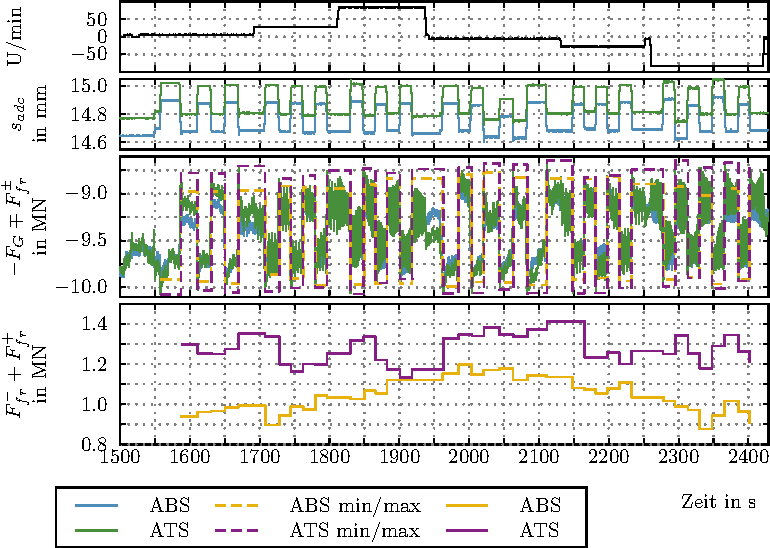
\includegraphics{fig_ExpVariationADC_WeightNFriction}
	\label{fig:WeightNFriction}
	\caption{Gewichtskraft und Reibkraft.}
\end{figure}


\section{Ausgangssituation und Aufgabenstellung}
Im Rahmen der Forschungskooperation zwischen der AG der Dillinger Hüttenwerke und dem Institut für Automatisierung- und Regelungstechnik (ACIN) der Technischen Universität Wien sollen Strategien zur Optimierung des Aufbaus und der Regelung der Richtspaltgeometrie von Warmrichtmaschinen entwickelt werden. Als konkretes Anwendungsbeispiel und  Ausgangspunkt der Untersuchungen dient dazu die Warmrichtmaschine P2 am Standort GTS in Dünkirchen.

%Das Richten von Walztafeln in einer Warmrichtmaschine soll abwickelbare und nicht-abwickel"=bare Ebenheitsdefekte zufolge von Resteigenspannungen reduzieren. Die Walztafel wird dazu wechselseitig über versetzt angeordnete Richtrollen gebogen und dabei gezielt plastifiziert. %Mit einem Richtprozessmodell wird die optimale Anstellung der Richtrollen berechnet und mittels einer elektromechanischen Voranstellung und positionsgeregelter Anstellzylinder eingestellt (vgl. Abb. \ref{fig:schema_aktor} links). Da die Richtmaschine unter der Wirkung der Richtkräfte auffedert, muss die berechnete Zustellung um die Auffederung korrigiert werden. Dabei ist neben der vertikalen Auf"|federung der Anstellschrauben die Querauf"|federung, d.\,h. die Durchbiegung der Richtrollen und die Auf"|federung des Druckrahmens, von Bedeutung.
%Die Richtmaschine federt unter der Wirkung der Richtkräfte auf. Um den gewünschten Richtspalt einzustellen, muss die mit einem Richtmodell berechnete Zustellung um die vertikale Auf"|federung der Anstellschrauben und insbesondere die Querauf"|federung, d.\,h. die Durchbiegung der Richtrollen und die Auf"|federung des Druckrahmens, korrigiert werden.


\begin{bemerkung}
	Eine Bemerkung
\end{bemerkung}

\begin{hinweis}
	Ein Hinweis
\end{hinweis}
Eine wichtige Formel
\begin{markeqn}
\begin{align}
1=1 \ .
\end{align}
\end{markeqn}

Hier folgen einige Literaturreferenzen, z.B. \cite{Henrich1993}
oder\cite{Witte1970}.

	% Include chapter bib for CDS publications
	\chapter{Literaturübersicht CDS-Publikationen}
\cite{AIT-140982} : Surface Following Control for Fully Actuated Rigid Body Systems in Three-Dimensional Euclidean Space
\\
\cite{AIT-142586} : Model-Based Signal Processing for the Force Control of Biaxial Grantry Robots
\\
\cite{AIT-142387} : Force-based cooperative handling and lay-up of deformable materials: Mechatronic design, modeling, and control of a demonstrator
\\
\cite{AIT-141890} : Path Following Control for Elastic Joint Robots
\\
\cite{AIT-141654} : Modeling and Control of the Oxygen Concentration in a Post Combustion Chamber of a Gas-Fired Furnace
\\
\cite{AIT-141651} : Combined Path Following and Compliance Control for Fully Actuated Rigid Body Systems in 3-D Space
\\
\cite{AIT-146558} : Convex Constrained Iterative Learning Control Using Projection: Application to a Smart Power Switch
\\
\cite{AIT-144111} : A Path/Surface Following Control Approach to Generate Virtual Fixtures
\\
\cite{AIT-144110} : Modelling, Estimation and Control Concepts for Pneumatic Systems
\\
\cite{AIT-144109} : Flatness-based nonlinear control of a three-dimensional gantry crane
\\
\cite{AIT-143622} : Mathematical Modelling and Advanced Process Control for Industrial Applications in the Steel Industry
\\
\cite{AIT-143052} : Control and estimation strategies for pneumatic drives with partial position information
\\
\cite{AIT-142969} : Hierarchical nonlinear optimization-based controller of a continuous strip annealing furnance
\\
\cite{AIT-146187} : Collaborative Synchronization of a 7-Axis Robot
\\
\cite{AIT-146186} : Optimal Current Slew Rate Control for a Three-Phase MOSFET Inverter Driving a PMSM
\\
\cite{AIT-146185} : Swing-Up of a Spherical Pendulum on a 7-Axis Industrial Robot
\\
\cite{AIT-146013} : Torque Control of a Hydrostatic Transmission Applied to a Wheel Loader
\\
\cite{AIT-145989} : Dynamic Virtual Fixtures Based on Path Following Control
\\
\cite{AIT-145984} : Improved EMD-based Oscillation Detection for Mechatronic Closed-Loop Systems
\\
\cite{AIT-145737} : Fortgeschrittene Methoden der nichtlinearen Regelung
\\
\cite{AIT-145690} : A dynamic model of power metal-oxide-semiconductor field-effect transistor half-bridges for the fast simulation of switching induced electromagnetic emissions
\\
\cite{AIT-145460} : Advanced Process Control in the Steel Industry
\\
\cite{AIT-144906} : AI - How will it change industrial automation?
\\
\cite{AIT-144905} : Advance model-based control for rolling of flat products
\\
\cite{AIT-146335} : Pfadfolgeregelung mit Konzepten f{\"u}r den Pfadfortschritt: Ein Assemblierungsszenario


	
	% Appendix...
	%=============
	\appendix
	%\include{./chapters/Grundlagen_Naehen}
	%\addcontentsline{toc}{chapter}{Literatur}
	\printbibliography
	
	% ===================
% ||   Contact   ||
% ===================
		\clearscrheadfoot
		\pagestyle{scrheadings}
		\sffamily

		\begin{center}
		\@ifundefined{tikz@library@external@loaded}{}{\tikzset{external/export=false}}
		\begin{tikzpicture}[remember picture,overlay,outer sep=0pt,inner sep=0pt]
		
\node [anchor=south west,xshift=7cm,yshift=2cm] at (current page.south west){
\begin{tabularx}{\textwidth}{c}
%\arrayrulecolor{purple}
\fontsize{12}{12}\bfseries\selectfont\color{ait_red}{\Contact} \\
\newline\\
\fontsize{9}{9}\selectfont\color{ait_gray}{AIT Austrian Institue of Technolgy GmbH}\\
\fontsize{9}{9}\selectfont\color{ait_gray}{Argentiniertra\ss e 2/4, 1040 Wien, \"Osterreich}\\
\newline\\
\fontsize{9}{9}\selectfont\color{ait_gray}{www.ait.ac.at}\\
\newline\\
\newline\\
\fontsize{9}{9}\bfseries\selectfont\color{ait_gray}{\insertAuthor}\\
\fontsize{9}{9}\selectfont\color{ait_gray}{\Jobdescription}\\
\fontsize{9}{9}\selectfont\color{ait_gray}{Center for Vision, Automation \& Control}\\
\fontsize{9}{9}\selectfont\color{ait_gray}{Complex Dynamcial Systems}\\
\fontsize{9}{9}\selectfont\color{ait_gray}{\Telefonnumber}\\
\fontsize{9}{9}\selectfont\color{ait_gray}{\Email}\\
\end{tabularx}};
\end{tikzpicture}
\end{center}



\end{document}
